% filename: HEP_GL_IPZ_FSS_Coldflow_OperationSafetyConcept

\documentclass{article}

\usepackage[utf8]{inputenc}
\usepackage[top=3cm, headheight=2.2cm, headsep=10pt]{geometry}
\usepackage{graphicx}

% To reference the last page
\usepackage{lastpage}

% Like `tabularx` but supports pagebreaks
\usepackage{ltablex}
% Adjust row vertical spacing
\renewcommand{\arraystretch}{1.2}

% Multiline cells
\usepackage{makecell}

% Set date format to ISO 8601
\usepackage{datetime}
\newdateformat{isodate}{\THEYEAR-\twodigit{\THEMONTH}-\twodigit{\THEDAY}}

% Table colouring
\usepackage[table,dvipsnames]{xcolor}
\definecolor{tableHeaderColor}
{rgb}{0.75,0.75,0.75}
\definecolor{tableColumnColor}
{rgb}{0.95, 0.95, 0.95}
\definecolor{notesColor}
{rgb}{0.95, 0.95, 0.95}
\definecolor{highlightColor}
{rgb}{1.00, 0.95, 0.80}

% Icons for checkbox
\usepackage{pifont}

% Command to create a checkbox
\newcommand{\checkbox}{\ding{113}}

% For automatic counters
\usepackage{array}

% Header and footer
\usepackage{fancyhdr}
\pagestyle{fancy}
\fancyhf{} % Clear header and footer
\renewcommand{\headrulewidth}{0pt}
\lhead{\includegraphics[width=2cm]{../../common/assets/HELIOS_LOGO.png}}
\rhead{\includegraphics[width=2cm]{../../common/assets/ARIS_space_to_grow_LOGO-black.pdf}}
\cfoot{\thepage}
\fancyfoot[L]{Project HEPHAESTUS}
\fancyfoot[C]{Page \thepage\ out of \pageref{LastPage}}

% Draft watermark
\newboolean{isDraft}
\setboolean{isDraft}{true} % Set to false to remove the watermark
\ifthenelse{\boolean{isDraft}}{
  \usepackage{background}
  \backgroundsetup{
    scale=25,
    color=gray,
    opacity=0.4,
    angle=45,
    position=current page.center,
    contents={Draft}
  }
}{}

% Highlight colour
\usepackage{soul}
\sethlcolor{magenta}

% Strikethrough
\usepackage[normalem]{ulem}

% Clickable Hyperlinks
\usepackage[colorlinks=true, linkcolor=blue, urlcolor=blue]{hyperref}

% Toggleable procedure items
\usepackage{etoolbox}



\title{IPZ FSS Coldflow Operation Safety Concept}
\author{Guideline}
\date{Version: \isodate\today}

\begin{document}

\maketitle

% Set the page style for the title page
\thispagestyle{fancy}

\section{Scope}

Within the framework of the ETH Focus Project HEPHAESTUS, fuel supply system (FSS) cold flows will be performed on the IPZ area. The purpose of a cold flow is to inject the propellants (seperately) without ignition, to check if the propellant supply system functions correctly under operating circumstances.  
\noindent
For the FSS cold flow only \textbf{distilled water} will be used. To ensure efficient and safe tests, this operational safety concept shall describe the test area and its available safety equipment and gives instructions on how to behave during procedures and in emergencies.

\section{Location of safety-relevant Institutions}
The contact information of the relevant safety institutions is listed in \ref{tab:safety-relevant-institutions}.
\begin{table}[h]
    \caption{Information of safety-relevant institutions}
    \label{tab:safety-relevant-institutions}
    \begin{tabularx}{0.9\textwidth}{|X|X|X|}
        \hline
        \rowcolor{tableHeaderColor} \textbf{Description} & \textbf{Address} & \textbf{Phone Number} \\ \hline
        Test Location & \begin{minipage}[t]{\linewidth}
            Innovationspark Zürich \\
            Wangenstrasse 68 \\
            8600 Dübendorf
            \vspace{1mm}
        \end{minipage} & +41 44 527 20 20 \\ \hline
        Spital Uster & \begin{minipage}[t]{\linewidth}
            Brunnenstrasse 42 \\
            8610 Uster
            \vspace{1mm}
        \end{minipage} & +41 44 911 11 11 \\ \hline
        President ARIS & Chloé Pilloud & +41 79 226 39 42 \\ \hline
    \end{tabularx}
\end{table}
\noindent
In table \ref{tab:emergency-numbers} the emergency numbers are listed. Call them first before calling other relevant security institutions. In the case of an emergency, follow the contingency procedures as described in Section \ref{emergency-behaviour}.
\begin{table}[h]
    \caption{Emergency Numbers}
    \label{tab:emergency-numbers}
    \begin{tabularx}{0.9\textwidth}{|X|X|}
        \hline
        \rowcolor{tableHeaderColor} \textbf{Description} & \textbf{Phone Number} \\ \hline
        Ambulance & 144 \\ \hline
        Rega & 1414 \\ \hline
        Fire service & 118 \\ \hline
        Police & 117 \\ \hline
        Toxics & 145 \\ \hline
    \end{tabularx}
\end{table}
\newpage
\section{Site Map}
The tests will be performed in the IPZ Test Area 2. The trailer will be positioned all the way at the fence to the airfield, with both the side of the system that will be pressurized and the engine compartment facing the airfield. The control station will be positioned close to the Hangar. The whole testing area will be taped off to prevent accidental trespassing and during pressurized operations a dedicated person will monitor the area to look out for trespassers.
Figure \ref{fig:location-plan} shows the setup of the test location and the location of the fire extinguisher and first aid kit. During active testing, only the test conductor, safety officer and engineer in charge are allowed inside the taped zone with appropriate safety equipment (safety goggles and ear protection). When the system is pressurized, no one is allowed inside the taped off safety zone.
The size of the safety zone was determined by calculating the TNT equivalent of the stored energy in the system and the resulting safety radius using the ASME PCC-2-2018 standard, the exact calculations can be found in the HEPHAESTUS safety folder on Sharepoint. The resulting minimal safety radius for a Water coldflow is 5 meters. To have added safety and because it's easier to tape off the quadratic test area, the entire test area, which has a radius of around 20 metres, is taped off and monitored during testing.
\begin{figure}[h]
    \centering
    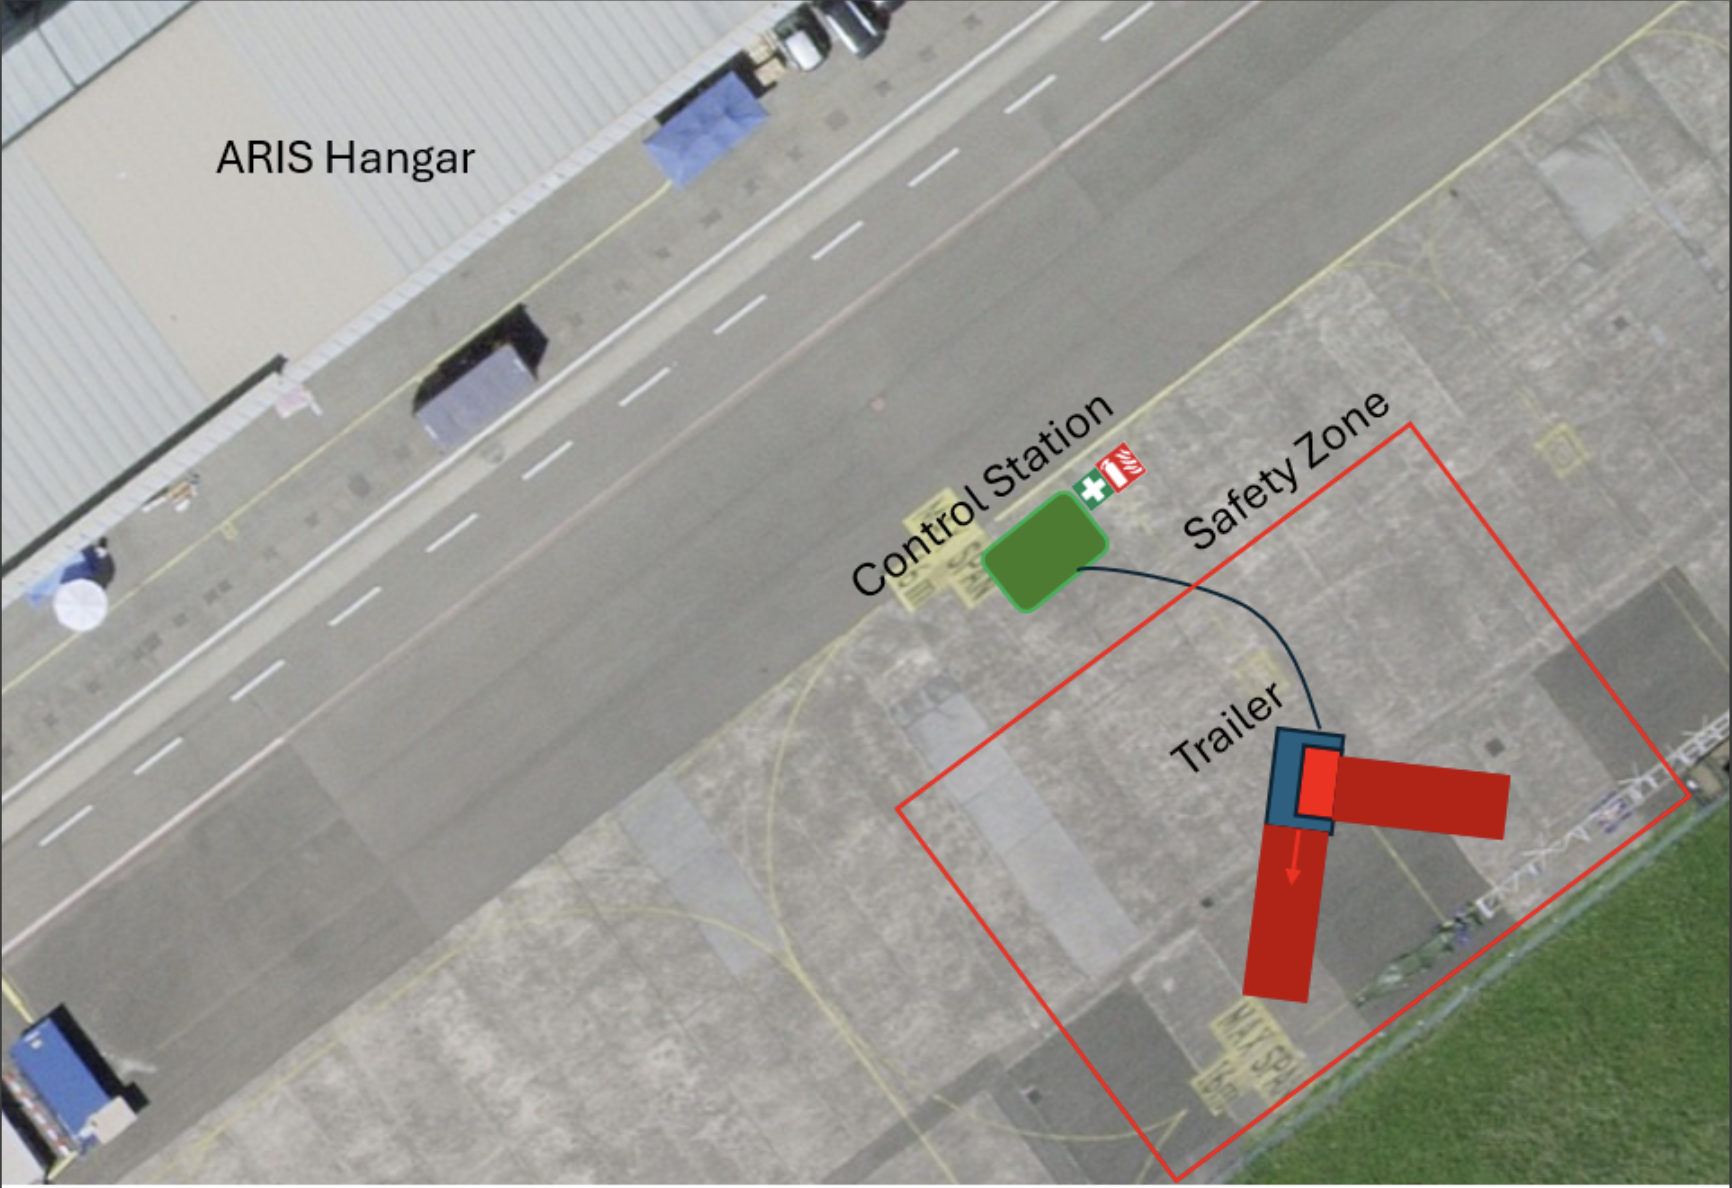
\includegraphics[width=0.7\textwidth]{assets/location-map.png}
    \caption{Site map of the test location}
    \label{fig:location-plan}
\end{figure}

\newpage

\newpage
\section{Equipment}
Every person has to wear a warning vest according to their role at all times during testing operations. The color code displayed in table \ref{tab:color-code} is used.
\begin{table}[h]
    \caption{Warning Vest Color Code}
    \label{tab:color-code}
    \begin{tabularx}{0.9\textwidth}{|X|X|X|X|}
        \hline
        \cellcolor{cyan} Test Conductor & \cellcolor{green} Safety Officer & \cellcolor{orange} Engineers in charge (determined in role assignment) & \cellcolor{yellow} Visitors \\ \hline
    \end{tabularx}
\end{table}
The safety equipment is stored inside the ARIS Hangar. The wearing of provided safety equipmentas foreseen in the operating procedures is mandatory.
\begin{table}[h]
    \caption{Safety Equipment}
    \label{tab:safety-equipment}
    \begin{tabularx}{0.9\textwidth}{|c|X|X|}
        \hline
        \rowcolor{tableHeaderColor} \textbf{Amount} & \textbf{Equipment} & \textbf{Comment} \\ \hline
        2 & Fire extinguisher & ABC-Pulver \\ \hline
        2 & Fire extinguisher & CO2 (class B next to trailer) \\ \hline
        1 & First aid kit &  \\ \hline
        2 & Blue warning vest & \\ \hline
        2 & Green warning vest & \\ \hline
        10 & Yellow warning vest & \\ \hline
        6 & Orange warning vest & \\ \hline
        8 & Safety goggles & \\ \hline
        4 & Face shield & \\ \hline
        6 & Pair of safety shoes & \\ \hline
        10 & Ear protection & \\ \hline
        8 & Work gloves & \\ \hline
        2 & Barrier tape & \\ \hline
    \end{tabularx}
\end{table}
\section{Behaviour during test procedure}
The test conductor has the lead during the whole test operation and therefore gives the orders, which shall be obeyed. The safety officer supervises the actions of the test conductor and the team and makes sure that the tests are executed according to the procedures. The safety officer can stop the operations at any time he considers proceeding with the test as dangerous. \\
\noindent
If during the test procedure an anomaly occurs or if there is an insecurity, the test participants are requested to inform the test conductor and the safety officer immediately.
\newpage
\section{Behaviour in case of an emergency} \label{emergency-behaviour}
In case of an emergency or an unexpected system state, the contingency procedures (shown in table \ref{tab:contingency-procedures}) must be followed. Participants will be informed about the location of the contingency procedures during the briefing and installation.
\begin{table}[h]
    \caption{Contingency Procedures}
    \label{tab:contingency-procedures}
    \begin{tabularx}{0.9\textwidth}{|X|}
        \cellcolor{blue} \textcolor{white}{General} \\ \hline
        HEP\_CP\_GEN\_Injury\_XX \\ \hline
        HEP\_CP\_GEN\_Fire\_XX \\ \hline
        HEP\_CP\_GEN\_Trespassing\_XX \\ \hline
        \cellcolor{orange} PSS \\ \hline
        HEP\_CP\_PSS\_Leakage\_XX \\ \hline
        HEP\_CP\_PSS\_Overpressure\_XX \\ \hline
        HEP\_CP\_PSS\_BottleValveAnomaly\_XX \\ \hline
        HEP\_CP\_PSS\_NoisesHissing\_XX \\ \hline
        \cellcolor{yellow} DACS \\ \hline
        HEP\_CP\_DACS\_PowerLoss\_XX \\ \hline
        HEP\_CP\_DACS\_ConnectionLoss\_XX \\ \hline
        HEP\_CP\_DACS\_ValveAnomalies\_XX \\ \hline
    \end{tabularx}
\end{table}
All attendees are guided to stay calm and to avoid panicking. In such a situation, communication needs to be reduced to the minimum / essential only. The safety officer or his substitute leads through all emergency situations supported by the test conductor. \\
\noindent
In any situation, the hazards must be considered before providing assistance.
\noindent
As soon as the situation allows it, the safety officer will inform IPZ and Chloé Pilloud (ARIS). 
\end{document}